\documentclass{article}
\usepackage{ctex}
\usepackage{amsmath}
\usepackage{amssymb}
\usepackage{graphicx}
\usepackage{wrapfig}
\usepackage{hyperref}

\graphicspath{ {./images/} }
\title{\textbf{人工智能导论\ 四子棋\ 实验报告}}
\author{陈庆之 2021011819}

\begin{document}
	\maketitle
	
	\section{总述}
	
	四子棋是一种智力游戏。两名玩家轮流在m行n列的棋盘上落子,每次落子后棋子会落到对应列顶部。若在某次落子后己方的四枚或更多棋子在横、竖、斜向上连成直线,那么这名玩家赢得游戏。若棋盘被填满且没有任何一名玩家获胜,那么算作平局。
	
	部分大小的棋盘有必胜策略。本作业为了阻止必胜策略的应用,额外添加一不可落子点。若棋子将落入不可落子点,改为落在不可落子点正上方。若不可落子点位于列顶且其下已满,则不能在本列落子。
	
	本次作业中,我们利用\textbf{Monte-Carlo}算法进行\textbf{信心上限树搜索},实现了四子棋AI程序。在Saiblo平台上,我们提交的AI达到了95\%胜率(在偶数编号标准AI上测试)。
	
	\section{实现方法}
	
	\subsection{Monte-Carlo树搜索}
	
	人类在进行棋类游戏时通常通过归纳总结行棋,即基于经验和逻辑推导分析出各个情况的优劣,然后选择自己认可的行动。但是,简单的AI模型通常不具备完备的类人的逻辑思维能力。如果局面较为简单,程序可以利用算力优势枚举每一种可能的情况并挑选其中最好的策略,但对于绝大多数足以被称为棋类运动的游戏,这样枚举出的决策树会指数级增长,枚举的复杂度是不可接受的。
	
	Monte-Carlo算法即反其道而行之,纯粹使用统计与概率的方式行棋直至比赛结束,将随机行棋的结果记录到各个着法上,并依据随机行棋的结果统计出“最可能获胜”的着法。只要随机行棋的次数足够多,大数定律就可以保证统计的结果基本收敛到着法的好坏。
	
	具体而言,对于每个局面$state$,我们定义其奖赏(reward)为:$reward = \frac{n_{\text{win}} - n_{\text{loss}}}{n_{\text{simulation}}}$, 其中win/loss/simulation分别对应当前局面下的胜利次数、失败次数和总模拟次数。注意,我们并不关心从当前局面出发之后,接下来的行棋过程是带有策略或筛选的,还是全部或部分随机挑选着法的。只要是完成了一次模拟并获得了最终结果,我们就记录到当前局面上。换言之,每个局面的记录都会回溯到决策树的根。
	
	\subsection{UCT}
	
	\textbf{信心上限树搜索}(\textbf{U}pper \textbf{C}onfidence bounds applied to \textbf{T}rees)是Monte-Carlo树搜索的优化版本。设想存在某一步坏棋,如果下出这步棋,那么对手有一些强制着法可以在若干步内获胜或者获得巨大优势,但如果对手错过了这些强制着法,那么我方可以轻易获胜。如果纯粹地按照Monte-Carlo树的方法随机落子,那么这步坏棋会因为“大多数”后续着法都对我方有利而被错误地评估为好棋,殊不知对手只要棋艺不是太差都能让我们立刻输掉游戏。实际上,在棋类游戏中这样的情形很常见:国际象棋有句名言“胜利者是犯下倒数第二个错误的人”,即说明很多时候一着不慎就可满盘皆输。
	
	针对这种情况,我们使用了UCT算法。它的核心思路是:每个局面的评估不再只与当前局面的胜率有关,还与当前局面的模拟次数有关。形式化地,设$n$为某个局面被模拟的次数,$w$为胜利次数,则每个子局面$j$的UCT值可表示为:
	
	\begin{equation}
		UCT = \frac{w_j}{n_j} + c\sqrt{\frac{\ln{n}}{n_j}}
	\end{equation}

	其中$c$为一常数,$c$越大则程序越倾向于探索访问较少的策略(更激进,不“安于现状”)。这样就可以提升Monte-Carlo过程的广度,尽可能减少前述情况。
	
	\subsection{实现}
	
	我们的算法流程大致如下:
	
	\begin{figure}[ht]
		\centering
		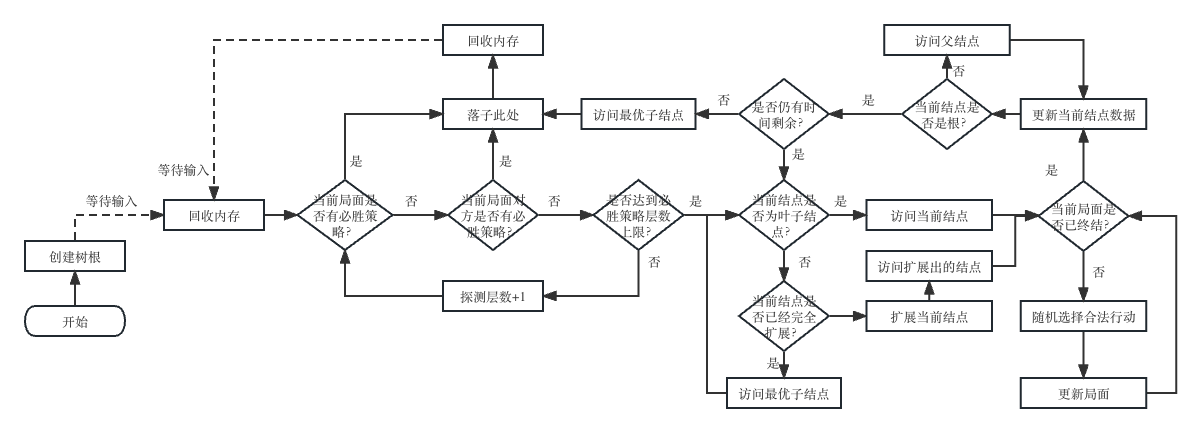
\includegraphics[width=0.9\textwidth]{procedure.png}
		\caption{四子棋算法流程}
	\end{figure}
	
\end{document}